\addbibresource{reference.bib}

\chapter{Úvod do hybridních částicových pixelových detektorů}\label{chap:detectors}
Ionizující záření je lidskými smysli nedetekovatelné, avšak jeho studie nám umožňuje pochopit podstatu hmoty, její vlastnosti a interakce. To lidstvu umožnilo mnohé aplikace, jako je na příklad protonová terapie, defektoskopie nebo zkoumání pravosti uměleckých děl. První pokusy o detekci ionizujícího záření sahají do počátku 20. století, kde pomocí mlžné komory se prvně podařilo zachytit trajektorii nabitých částic. Rozvoj polovodičové technologie dal vzniku novým detekčním technologiím až po v současné době nejpokrokovějším - pixelovým detektorům.

Existuje celá řada částicových pixelových detektorů, ale v této kapitole budou popsány jen hybridní pixelové detektory, pro které je typické, že se skládají ze dvou nezávisle vyrobených částí - senzoru a vyčítacího čipu. To oproti monolitickým detektorů, kde vyčítací elektronika je součástí senzoru přináší řadu výhod, jako na příklad snížení výrobních nákladů nebo možnost kombinace vyčítacího čipu se senzory různých materiálů (\textit{Si}, \textit{GaAs}, \textit{CaTe} apod.).

Na tomto místě je třeba zmínit, že existuje více druhů těchto detektorů (\textit{AGH Fermilab, Pilatus, Philips Chromaix} apod.)\cite{detectors_review}, v této práci budou použity použity pouze detektory z rodiny detektorů Medipix.


\section{Hardwarová architektura}
\begin{figure}[th]
	\begin{center}
		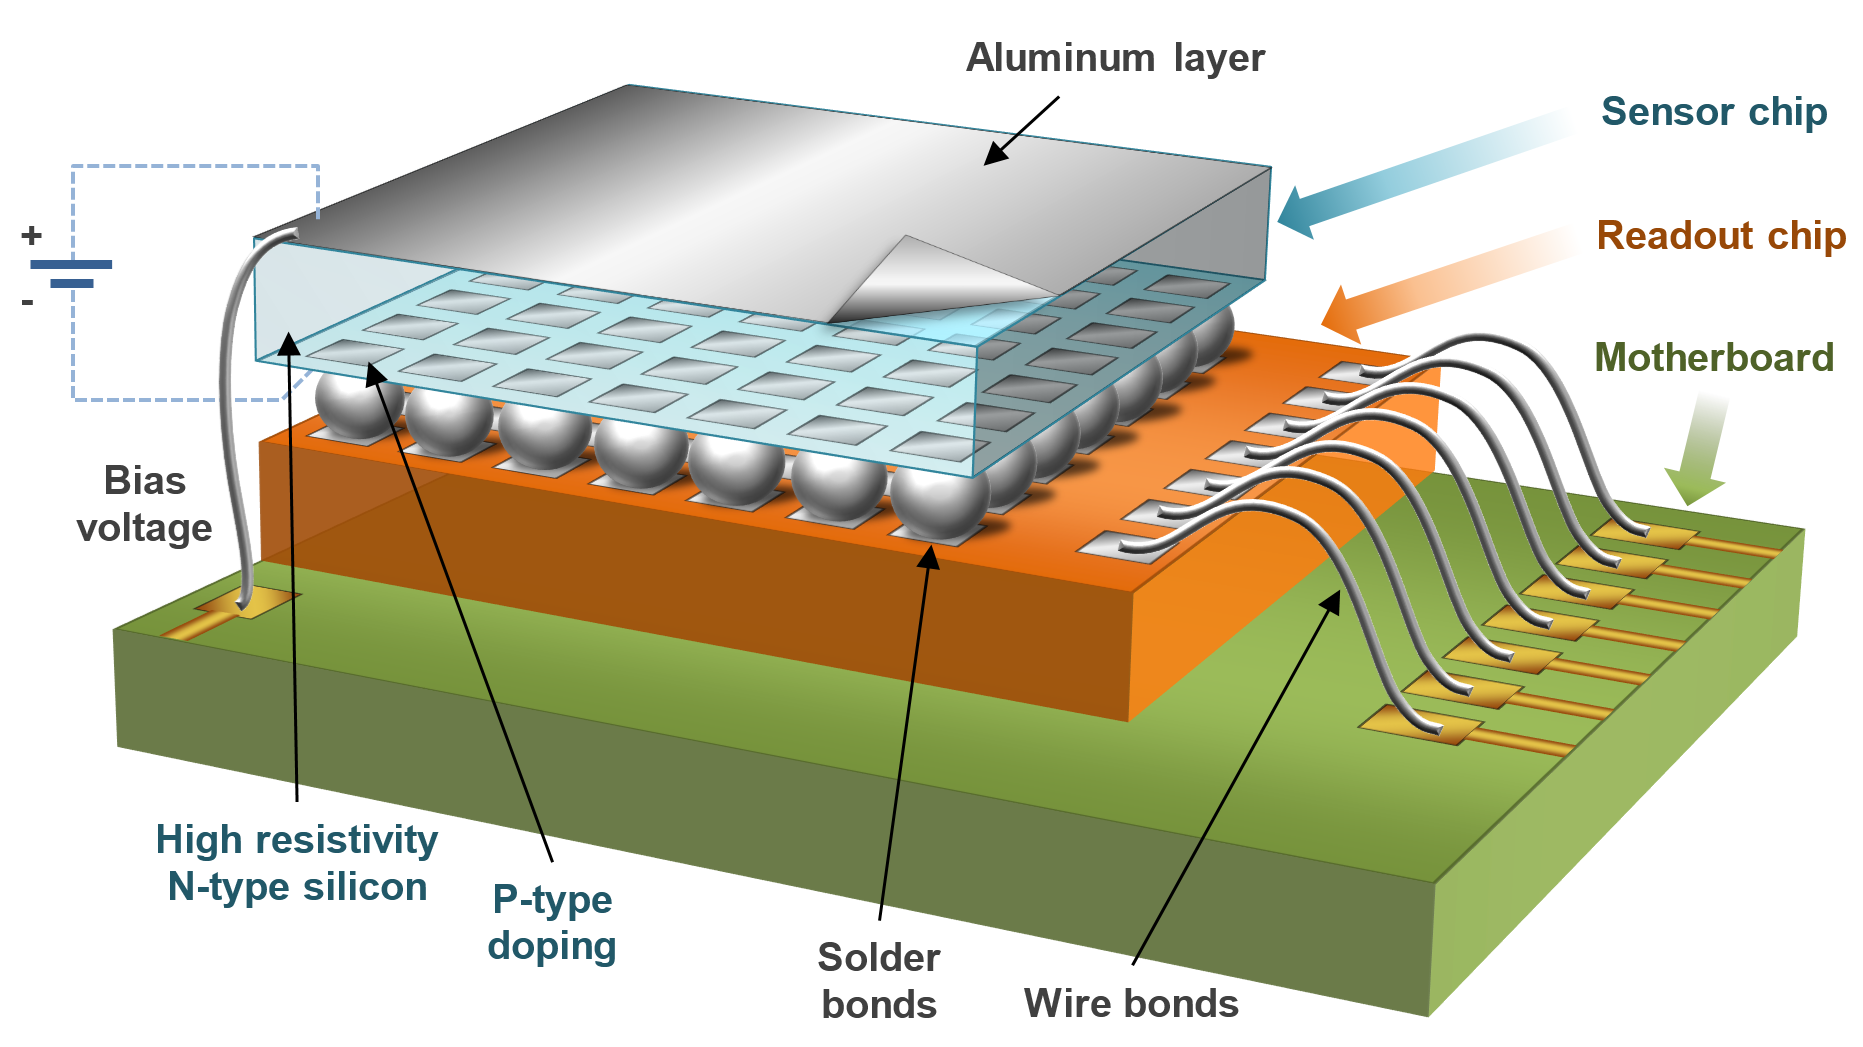
\includegraphics[width=12cm]{figures/det_chip.png}
		\caption{Struktura hybridního polovodičového pixelového detektoru Timepix3, skládající se z vyčítacího čipu a polovodičového senzoru (převzato z~\cite{PlatkevicDisertace}).}
		\label{fig:det:chip}
	\end{center}
\end{figure}
Většina hybridních částicových pixelových detektorů rodiny Medipix obsahuje matici $256\times256$ pixelů. Každý z nich má stanu o délce $55~\mu m$, takže senzor čítající $65536$ má plochu $1.4 \times 1.4 cm^2$. 

Na obrázku \ref{fig:det:chip} je znázorněna struktura detektoru Timepix3. Vrchní část detektoru tvoří polovodičový senzor, který je nejčastěji vyroben z křemíku, ale výjimkou není také \textit{GaAs} nebo \textit{CaTe}. Jednotlivé pixely senzoru jsou spojeny s integrovaným \texttt{ASIC}\footnote{z angl. Application Specific Integrated Circuit} vyčítacím čipem pomocí technologie zvané \textit{Bump-Bounding}. Vyčítací čip je pak propojen se základní deskou pomocí \textit{wire-bound}, z které je ještě přivedeno měřící napětí na senzor detektoru (tzv. \textit{bias}).


\section{Princip detekce}
\begin{figure}[th]
	\begin{center}
		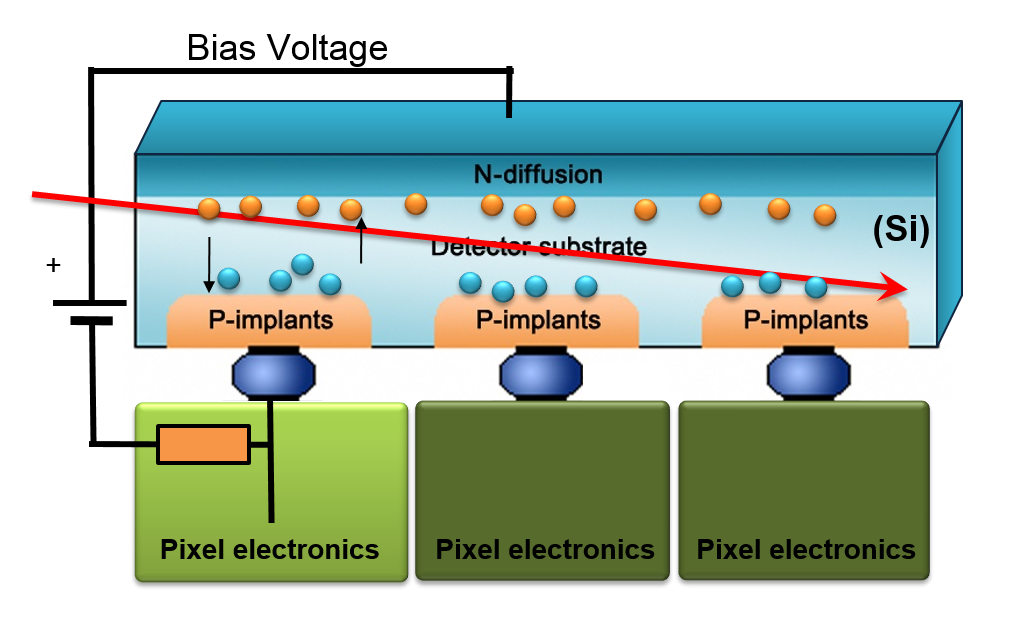
\includegraphics[width=10cm]{figures/det_recombination.png}
		\caption{Princip detekce ionizujícího záření detektorem Timepix3 (převzato z~\cite{PlatkevicDisertace}).}
		\label{fig:det:recombination}
	\end{center}
\end{figure}

Princip detekce ionizujícího záření pixelovými detektory je založen na známém jevu detekce ionizujícího záření v polovodiči. 

Jako náhradní schéma jednoho pixelu si lze představit diodu zapojenou v závěrném směru, kterou bez přítomnosti ionizujícího záření protéká minimální proud. Vnikne-li do senzoru ionizující částice a dojde k její interakci se senzorem, resp. část její energie je deponována do polovodičového objemu senzoru, dojde v senzoru ke vzniku elektron-děrových páru a díky lavinovému efektu i k následnému otevření PN přechodu (viz. na obr. \ref{fig:det:recombination}, kde červená šipka znázorňuje interagující částici, elektrony jsou znázorněny žlutě, modře díry).

Vzniklý proudový impulz je měřícím odporem převeden na napětí, které je komparátorem porovnáno s prahovým napětím (tzv. \textit{threshold}). Výsledek této komparace je dále CMOS obvodem zpracován, dle použitého měřícího módu, jak bude ukázáno v kapitole \ref{chap:detectors:operation_modes}.

Na rozdíl od CCD technologii, \textit{Timepix}/\textit{Medipix} detektory není generován temný proud\footnote{Termín charakterizující vyčítací šum u CCD snímačů. Obvykle je udáván v elektronech za sekundu při konstantní teplotě a ve tmě.}, díky odstínění signálu od šumu pomocí komparačního napětí. To znamená, že doba jedná akvizice je teoreticky neomezena, protože detektor je schopný detekovat jen ty částice, jejíchž deponovaná energie (resp. amplituda vzniklého napěťového pulzu) je větší, než \textit{threshold}.

\section{Operační módy detektoru}\label{chap:detectors:operation_modes}
V této podkapitole bude vysvětlena většina operačních módu, ve kterých detektory rodiny \textit{Medipix} jsou schopny pracovat.